% ============================================================
%  MATH & DATA SCIENCE REPORT TEMPLATE
%  Customisation guide is inline — search for [EDIT] tags
% ============================================================

% ── [EDIT] Document class ───────────────────────────────────
% Options: 11pt / 12pt  |  a4paper / letterpaper  |  twoside
\documentclass[12pt, a4paper, onecolumn]{article}


% ╔══════════════════════════════════════════════════════════╗
% ║  PACKAGES                                                ║
% ╚══════════════════════════════════════════════════════════╝

% ── Layout & Typography ─────────────────────────────────────
\usepackage[
  top=2.5cm, bottom=2.5cm,
  left=2.5cm, right=2.5cm,   % [EDIT] margins
  headheight=14pt
]{geometry}

\usepackage{microtype}        % Better text justification (keep this!)
\usepackage{parskip}          % Space between paragraphs instead of indent
                              %   Remove for classical indented paragraphs

% ── [EDIT] Font choice (uncomment ONE block) ─────────────────
% -- Option A: Computer Modern (LaTeX default, no package needed)
%    Just leave all font blocks commented out.

% -- Option B: Times-like (common in journals)
% \usepackage{mathptmx}

% -- Option C: Palatino (elegant, easy to read)
\usepackage[sc]{mathpazo}
\linespread{1.05}
% \usepackage{charter}

% -- Option D: Latin Modern (improved CM, recommended default)
% \usepackage{lmodern}
\usepackage[T1]{fontenc}
\usepackage[utf8]{inputenc}   % UTF-8 source encoding

% ── Maths ───────────────────────────────────────────────────
\usepackage{amsmath}          % align, gather, split, cases, ...
\usepackage{amssymb}          % \mathbb, \mathcal, extra symbols
\usepackage{amsthm}           % theorem / proof environments
\usepackage{mathtools}        % extends amsmath (coloneqq, :=, etc.)
\usepackage{bm}               % bold math: \bm{x}
\usepackage{bbm}              % blackboard bold digits: \mathbbm{1}

% ── Statistics & Data Science symbols ───────────────────────
\usepackage{dsfont}           % \mathds{1}  indicator function

% ── Algorithms ──────────────────────────────────────────────
\usepackage[ruled, vlined, linesnumbered]{algorithm2e}
% [EDIT] options: ruled/boxed/plain  |  vlined/lined  |  linesnumbered

% ── Figures & Plots ─────────────────────────────────────────
\usepackage{graphicx}         % \includegraphics
\usepackage{float}            % [H] placement
\usepackage{caption}
\usepackage{subcaption}       % subfigures side by side
\usepackage{tikz}             % programmatic figures
\usepackage{pgfplots}         % data plots inside LaTeX
\pgfplotsset{compat=1.18}
\usetikzlibrary{arrows.meta, positioning, shapes, calc}

% ── Tables ──────────────────────────────────────────────────
\usepackage{booktabs}         % \toprule, \midrule, \bottomrule
\usepackage{tabularx}         % auto-width columns (X type)
\usepackage{multirow}         % \multirow
\usepackage{array}            % extra column formats

% ── Code listings ───────────────────────────────────────────
\usepackage{listings}
\usepackage{xcolor}

% [EDIT] Colour scheme for code
\definecolor{codebg}{HTML}{F7F7F7}
\definecolor{codeframe}{HTML}{CCCCCC}
\definecolor{codekw}{HTML}{0000CC}
\definecolor{codecomment}{HTML}{008000}
\definecolor{codestring}{HTML}{AA0000}

\lstdefinestyle{mycode}{
  backgroundcolor = \color{codebg},
  frame           = single,
  rulecolor       = \color{codeframe},
  basicstyle      = \ttfamily\small,
  keywordstyle    = \color{codekw}\bfseries,
  commentstyle    = \color{codecomment}\itshape,
  stringstyle     = \color{codestring},
  numbers         = left,
  numberstyle     = \tiny\color{gray},
  numbersep       = 6pt,
  breaklines      = true,
  showstringspaces= false,
  tabsize         = 4,
}
\lstset{style=mycode}
% Usage: \begin{lstlisting}[language=Python] ... \end{lstlisting}

% ── Hyperlinks & Cross-references ───────────────────────────
\usepackage[
  colorlinks = true,
  linkcolor  = NavyBlue,    % internal links  [EDIT]
  citecolor  = BrickRed,    % citations        [EDIT]
  urlcolor   = NavyBlue,    % URLs             [EDIT]
  bookmarks  = true,
  pdfusetitle
]{hyperref}
\usepackage[dvipsnames]{xcolor}   % named colours (load before hyperref if clashing)
\usepackage{cleveref}             % \cref{} — smart "Figure 1", "Eq. (2)", …

% ── Bibliography ────────────────────────────────────────────
\usepackage[
  backend  = biber,        % [EDIT] bibtex also works: backend=bibtex
  style    = numeric,      % [EDIT] try: authoryear, apa, ieee, alphabetic
%   sorting  = nyt,
  sorting = none,
  maxnames = 3
]{biblatex}
\addbibresource{references.bib}   % [EDIT] your .bib filename

% ── Miscellaneous ───────────────────────────────────────────
\usepackage{enumitem}       % fine-grained list control
\usepackage{lipsum}         % dummy text (\lipsum[1-3])
\usepackage{todonotes}      % \todo{fix this}  margin notes
\usepackage{siunitx}        % SI units: \SI{3.2e-4}{\metre\per\second}
\usepackage{csquotes}       % \enquote{text}  (also needed by biblatex)


% ╔══════════════════════════════════════════════════════════╗
% ║  THEOREM ENVIRONMENTS                                    ║
% ╚══════════════════════════════════════════════════════════╝
% [EDIT] Add / remove / rename environments freely

\theoremstyle{plain}          % italic body
\newtheorem{theorem}{Theorem}[section]
\newtheorem{lemma}[theorem]{Lemma}
\newtheorem{proposition}[theorem]{Proposition}
\newtheorem{corollary}[theorem]{Corollary}

\theoremstyle{definition}     % upright body
\newtheorem{definition}[theorem]{Definition}
\newtheorem{example}[theorem]{Example}

\theoremstyle{remark}
\newtheorem*{remark}{Remark}
\newtheorem*{note}{Note}


% ╔══════════════════════════════════════════════════════════╗
% ║  CUSTOM COMMANDS — add your own below                    ║
% ╚══════════════════════════════════════════════════════════╝

% Probability & Expectation
\newcommand{\E}{\mathbb{E}}          % Expectation
\newcommand{\Prob}{\mathbb{P}}       % Probability
\newcommand{\Var}{\operatorname{Var}}
\newcommand{\Cov}{\operatorname{Cov}}

% Common sets
\newcommand{\R}{\mathbb{R}}
\newcommand{\N}{\mathbb{N}}
\newcommand{\Z}{\mathbb{Z}}
\newcommand{\C}{\mathbb{C}}

% Vectors & matrices  (bold lower/upper case)
\newcommand{\vx}{\bm{x}}
\newcommand{\vy}{\bm{y}}
\newcommand{\vz}{\bm{z}}
\newcommand{\mA}{\bm{A}}
\newcommand{\mB}{\bm{B}}

% Norms
\newcommand{\norm}[1]{\left\lVert #1 \right\rVert}
\newcommand{\abs}[1]{\left\lvert #1 \right\rvert}

% Indicator function
\newcommand{\Ind}[1]{\mathds{1}\!\left[#1\right]}

% argmin / argmax
\DeclareMathOperator*{\argmin}{arg\,min}
\DeclareMathOperator*{\argmax}{arg\,max}


% ╔══════════════════════════════════════════════════════════╗
% ║  HEADER & FOOTER  (fancyhdr)                             ║
% ╚══════════════════════════════════════════════════════════╝
\usepackage{fancyhdr}
\pagestyle{fancy}
\fancyhf{}
\fancyhead[L]{\small\leftmark}           % section name on left   [EDIT]
\fancyhead[R]{\small\textit{Duc Kien Doan}}  % [EDIT] your name or course
\fancyfoot[C]{\thepage}                  % page number centred
\renewcommand{\headrulewidth}{0.4pt}


% ╔══════════════════════════════════════════════════════════╗
% ║  TITLE BLOCK                                             ║
% ╚══════════════════════════════════════════════════════════╝
% [EDIT] Fill in your details

\title{
  \vspace{-1cm}
  {\Large \textsc{NUMERICAL MODELLING AND OPTIMIZATION}} \\[0.4em]
  \rule{\linewidth}{0.5pt} \\[0.6em]
  {\LARGE \bfseries Image Deblurring: A comparison between Classical and Modern Approaches} \\[0.3em]
  {\large Minicourse project report \\ Image restoration: from model to learning based techniques \\ (Lecturer: Mauro Dalla Mura - INP Grenoble)} \\[0.3em]                 % subtitle
  \rule{\linewidth}{0.5pt}
}

\author{
  Duc Kien DOAN \\                   % [EDIT]
  \small Matricola Number: VR543321 \\        % [EDIT]
  \small \texttt{duckien.doan@studenti.univr.it}  % [EDIT]
}

\date{
  \small September 2026                    % or: \small June 2025
}


% ╔══════════════════════════════════════════════════════════╗
% ║  DOCUMENT BODY                                           ║
% ╚══════════════════════════════════════════════════════════╝
\begin{document}

% ── Title page ──────────────────────────────────────────────
\maketitle
\thispagestyle{empty}     % no header/footer on title page

% ── Abstract ────────────────────────────────────────────────
\begin{abstract}
  \noindent
  Image deblurring is an ill-posed inverse problem requiring careful regularization to balance the reconstruction of the image and noise suppression. This report presents  comparison between classical spectral filtering methods and modern approaches (model-based, data-driven and hybrid) across degradation scenarios with two level of difficulty. Our experiments show that classical Generalized Tikhonov regularization with a Laplacian prior achieves the best pixel-wise and structural fidelity among model-based methods at negligible computational cost. Meanwhile, learned image priors are better at perceptual quality: Plug-and-Play (DPIR) yields superior structural preservation, while diffusion-based restoration (DiffPIR) achieves the best perceptual realism (LPIPS). We also highlight the critical dependence of classical methods on boundary condition mismatches, thus providing some guidelines for selecting the appropriate deblurring paradigm based on application constraints.
\end{abstract}

\newpage

% ── Table of contents ───────────────────────────────────────
\tableofcontents
\newpage

\section{Introduction}
% ============================================================
Inverse problems, a class of problems which takes a processed or altered image and aims to recover the original image, plays a very important role in several fields such as astrophysics, medicine and geosciences. One of them is image deblurring, where the problem is recovering a sharp image from a blurred, noisy image. The forward operation, blurring is defined to be a linear transformation that transforms an image $x$ to the blurred version $b$: 

\begin{equation}
    b = Ax + e,
    \label{eq:forward}
\end{equation}
where $A$ is a large, structured matrix representing convolution with a Point Spread Function (PSF), and $e$ is measurement noise. Because blurring
is a smoothing operation, $A$ is severely ill-conditioned: its singular values decay toward zero, so naive inversion $x = A^{-1}b$ catastrophically
amplifies noise in the components corresponding to fine image detail. Solving this problem requires regularization, which imposes a desirable structure of the image. This report compares classical and modern approaches to this problem, namely:

\begin{itemize}
    \item \textbf{Classical spectral filtering} (presented in the book \textit{Deblurring Images: Matrices, Spectra, and Filtering} \cite{hno2006}, denoted as \emph{HNO} from this point):
    Tikhonov regularization and Truncated Singular Value Decomposition (TSVD), made computationally tractable via
    fast transforms that take advantage of a chosen boundary-condition assumption.
    \item \textbf{Modern methods} implemented in the \texttt{DeepInverse}
    \cite{deepinv2023} Python package: explicit non-quadratic priors (Total Variation,
    wavelet sparsity) solved with iterative optimization algorithms like ADMM, Plug-and-Play priors using a
    pretrained denoiser (DPIR \cite{dpir2021}), and diffusion-model-based
    posterior sampling (DiffPIR \cite{diffpir2023}).
\end{itemize}

Both classes of method use the same problem formulation, which is solving the inverse problem of \ref{eq:forward} with regularization. This makes them directly
comparable, but they differ sharply in how they encode prior knowledge about natural images, in their computational cost, in how they perform across different evaluation metrics. Every method \emph{implemented and benchmarked} in this report, classical or modern, solves the \textit{non-blind deconvolution problem}, in which we
assume the PSF is known. This means the matrix $A$ is also known, so the focus is on solving an optimization problem to find $x$.

\textbf{Structure of this report.} Section~\ref{sec:background} rebuilds
the mathematical framework common to every classical method: the forward model, the ill-posedness argument, spectral filtering, and the role of boundary conditions in enabling fast computation. Section~\ref{sec:methods} focuses on the mathematical details of classical and modern methods. Section~\ref{sec:experiments} presents the experiment setup, evaluation metrics, and finally experiment results and discussion.

% ============================================================
\section{Mathematical Background}
\label{sec:background}
% ============================================================

\subsection{The forward model as discrete convolution}

For a 1D signal $x = (x_1,\dots,x_n)^T$ blurred by a PSF $h$ (assumed
centered, i.e.\ $h = (\dots,h_{-1},h_0,h_1,\dots)$ with $h_0$ the peak), the
blurred signal $b$ is the discrete convolution where
\begin{equation}
    b_i = \sum_k h_k\, x_{i-k}.
    \label{eq:conv}
\end{equation}
Writing $b = Ax$, row $i$ of $A$ contains the PSF weights centered at
position $i$: $A_{ij} = h_{i-j}$ whenever this index is in range. For
interior pixels this is unambiguous; for pixels near the boundary,
Equation~\eqref{eq:conv} calls for samples $x_{i-k}$ that fall outside
$\{1,\dots,n\}$, and \emph{what value is substituted there} is exactly the
boundary-condition choice discussed in Section~\ref{sec:bc}. Together, the boundary condition and the PSF determine the structure of matrix $A$. In 2D, if the
PSF is separable ($h(x,y) = h_{\text{row}}(x)\,h_{\text{col}}(y)$), the
blurring matrix has Kronecker structure $A = A_{\text{col}} \otimes
A_{\text{row}}$; if not, $A$ is block-Toeplitz-with-Toeplitz-blocks (or the
periodic/reflexive analogue) and no such compact factorization exists.

\subsection{Boundary conditions and the structure of $A$}
\label{sec:bc}

In reality, images are finite, but the convolution operation requires infinite functions, so the PSF's reach beyond the image border must be modeled by a \emph{boundary condition} (BC), an assumption about the image content outside the given frame. The BC choice directly determines the structure of $A$:

\begin{itemize}
    \item \textbf{Zero BC:} everything outside the image is assumed black. Row $i$ of $A$ simply omits (rather than substitutes) any PSF
    weight that would reach past the border. Therefore, in this case, the matrix $A$ is
    \textbf{Toeplitz}: constant along diagonals, with no wrap-around and no
    reflection.
    \item \textbf{Periodic BC:} the image is assumed to repeat infinitely like a periodic function, i.e. 
    the left edge is adjacent to the right edge (and similar in top to bottom).
    Out-of-range indices in Equation~\eqref{eq:conv} wrap around modulo
    $n$. The resulting $A$ is \textbf{circulant} (block-circulant-with-circulant-blocks,
    BCCB, in 2D): every row is a cyclic shift of the row above it.
    \item \textbf{Reflexive (Neumann) BC:} the image is assumed to be
    mirrored at its edges. Out-of-range indices are reflected back into
    range. The resulting $A$ is \textbf{Toeplitz plus Hankel},
    $A = T+H$: the Toeplitz part matches the zero-BC matrix, and the
    Hankel part is a low-rank correction capturing the reflected
    contributions near the corners.
\end{itemize}

\begin{table}[H]
\centering
\footnotesize
\begin{tabular}{p{1.5cm}p{3.3cm}p{3cm}p{5.5cm}}
\toprule
\textbf{BC} & \textbf{Assumption outside the image} & \textbf{Matrix structure} & \textbf{Typical edge accuracy} \\
\midrule
Zero & Black (value 0) & Toeplitz & Poor (dark ringing near borders) \\
Periodic & Wraps to opposite edge & Circulant & Poor (wrap-around discontinuity) \\
Reflexive & Mirrored at the edge & Toeplitz + Hankel & Best of the three for typical photographs \\
\bottomrule
\end{tabular}
\caption{Boundary conditions and the matrix structures they induce. See
Section~\ref{sec:classical-fast} for how each structure is exploited
computationally.}
\label{tab:bc}
\end{table}

Table \ref{tab:bc} shows that the choice of BC is not just a mathematical convenience, it introduces specific modeling errors at the borders that propagate inward during inversion. The zero BC assumes the image fades to black, which is rarely true. The periodic BC assumes the opposite edges match, which only happens by coincidence. The reflexive (mirroring) BC generally introduces the fewest artifacts for natural images, as pixel intensities tend to change smoothly near the borders.

Throughout this report, the blurring operator $A$ (and thus the PSF $h$ and the boundary conditions) is assumed to be known. We do not attempt to estimate the PSF from the blurred image $b$. This non-blind deconvolution assumption is shared by all the classical and modern methods evaluated here.

% ============================================================
\section{Methods}
\label{sec:methods}
% ============================================================

Given the shared forward model $b=Ax+e$ and matrix structure discussed in Section~\ref{sec:background}, this section presents the details of classical and modern methods. Both address the same underlying
ill-posedness, $A$'s small singular values make naive inversion amplify the noise, but they tackle this problem differently:

\begin{itemize}
    \item \textbf{The classical view} writes the solution directly as a \emph{filtered
    expansion} in the SVD basis of $A$, $x_{\text{reg}} = \sum_i \phi_i\,
    (u_i^Tb/\sigma_i)\,v_i$, choosing filter factors $\phi_i$ in closed form and evaluating the sum efficiently by exploiting the
    boundary-condition structure of Section~\ref{sec:bc}.
    \item \textbf{The modern view} instead formulates deblurring as an
    explicit \emph{optimization problem}, $\min_x \|Ax-b\|_{2}^2 + R(x)$, for
    a possibly non-quadratic or even implicit regularizer $R$, and solves it with a general-purpose iterative algorithm rather than a closed-form spectral filter.
\end{itemize}

As we can see later, the classical view is a special case of the modern one. Specifically, Tikhonov regularization is exactly $R(x)=\alpha^2\|x\|_2^2$, solved in
closed form because it is possible in this case. The modern methods
differ from the classical ones in choosing an $R$ or a denoiser/generative model that plays the role of $R$ implicitly. In such cases, no closed-form filtered solution exists, which calls for optimization algorithms.

\subsection{Classical methods: the filtered-solution view}
\label{sec:classical}

\subsubsection{Ill-posedness and spectral filtering}
\label{sec:filtering}

Let $A$ have the SVD $A=U\Sigma V^T=\sum_i \sigma_i u_i v_i^T$, with
singular values ordered $\sigma_1\ge\sigma_2\ge\dots\ge0$. The naive
least-squares solution to Equation~\eqref{eq:forward} is
\begin{equation}
    x_{\text{naive}} = A^{-1}b
    = \sum_i \frac{u_i^Tb}{\sigma_i}\,v_i
    = \underbrace{\sum_i \frac{u_i^TAx}{\sigma_i}\,v_i}_{=\,x}
    + \sum_i \frac{u_i^Te}{\sigma_i}\,v_i.
    \label{eq:naive}
\end{equation}
The first term reconstructs $x$, while the second
is essentially the noise, scaled by $1/\sigma_i$. Because blurring operators are smoothing operators, $\sigma_i$ decays, often exponentially for a
Gaussian PSF, toward the fine-detail (high-frequency) end of the
spectrum, so $1/\sigma_i$ grows very large exactly where the noise-free reference signal is weakest. This is the reason why deblurring is
\emph{ill-posed}: the solution does not depend continuously on the data.

The classical approach replaces Equation~\eqref{eq:naive} with a \emph{filtered} solution,
\begin{equation}
    x_{\text{reg}} = \sum_i \phi_i\,\frac{u_i^Tb}{\sigma_i}\,v_i,
    \qquad \phi_i\in[0,1],
    \label{eq:filtered}
\end{equation}
where the filter factors $\phi_i$ mitigate the dangerous small-$\sigma_i$ terms while leaving well-determined components ($\sigma_i\gg$ noise level)
close to untouched. The two classical strategies compared in this report differ only in how $\phi_i$ is computed:

\paragraph{Tikhonov regularization.} Solves the penalized least-squares problem
\begin{equation}
    \min_x\; \|Ax-b\|_2^2 + \alpha^2\|x\|_2^2,
    \label{eq:tik-problem}
\end{equation}
whose normal equations $(A^TA+\alpha^2I)x=A^Tb$ have closed-form solution in the SVD basis with filter factors
\begin{equation}
    \phi_i^{\text{Tik}} = \frac{\sigma_i^2}{\sigma_i^2+\alpha^2}.
    \label{eq:tik-filter}
\end{equation}
This means $\phi_i\approx1$ when $\sigma_i\gg\alpha$
(trusted components pass through) and $\phi_i\to0$ smoothly as
$\sigma_i\to0$. Statistically, this is the MAP estimate under a Gaussian
prior $x\sim\mathcal N(0,\tau^2I)$ and Gaussian noise, with
$\alpha^2=\text{noise variance}/\tau^2$ i.e.\ it encodes a generic
"smoothness/small-norm" belief about $x$, not anything specific to natural
images. Note that Equation~\eqref{eq:tik-problem} is already of the
optimization form $\min_x\|Ax-b\|_2^2+R(x)$ that Section~\ref{sec:modern}
generalizes; Tikhonov is the special case $R(x)=\alpha^2\|x\|_2^2$ with a closed-form solution.

\paragraph{Generalized Tikhonov with Laplacian regularization.}
While standard Tikhonov regularization penalizes the squared $\ell_2$ norm of the solution, $\alpha^2\|x\|_2^2$, which uniformly damps all frequency components and leads to the well-known over-smoothing of edges, \emph{generalized Tikhonov} regularization replaces this penalty with $\alpha^2\|Lx\|_2^2$, where $L$ is a user-specified regularization operator. The resulting optimization problem,
\begin{equation}
  \min_{x} \left\{ \|Ax - {b}\|_2^2 + \alpha^2 \|Lx\|_2^2 \right\},
\end{equation}
admits a closed-form solution $x_{\alpha} = (A^TA + \alpha^2 L^TL)^{-1}A^T{b}$. When $L$ is chosen as a discrete derivative operator, the penalty allows for variation: smooth regions incur little cost, while noise-like oscillations are heavily penalized. A particularly effective choice is the Laplacian operator,
\begin{equation}
    L = \begin{pmatrix} 0 & 1 & 0 \\ 1 & -4 & 1 \\ 0 & 1 & 0 \end{pmatrix},
\end{equation}
which penalizes the squared magnitude of the discrete second derivative and therefore preserves sharp edges while still suppressing noise.

Under reflexive boundary conditions, both the blurring matrix $A$ and the convolution operator $L$ are simultaneously diagonalized by the 2D Discrete Cosine Transform (DCT - presented in detail in section \ref{sec:classical-fast}): $A = C^T\Lambda_A C$ and $L = C^T\Lambda_L C$. The solution then decouples into independent scalar problems in the spectral domain,
\begin{equation}
    \hat{x}_k = \frac{\lambda_k^{(A)}}{\left(\lambda_k^{(A)}\right)^2 + \alpha^2 \left(\lambda_k^{(L)}\right)^2}\;\hat{b}_k,
\end{equation}
with corresponding filter factors
\begin{equation}
    f_k^{\text{GTik}} = \frac{\left(\lambda_k^{(A)}\right)^2}{\left(\lambda_k^{(A)}\right)^2 + \alpha^2 \left(\lambda_k^{(L)}\right)^2}.
\end{equation}
Because the Laplacian eigenvalues $\lambda_k^{(L)}$ are small at low frequencies (smooth components) and grow at high frequencies (edges and noise), the filter factors remain close to unity for low-frequency signal, pass through intermediate values near edges, and decay toward zero for noise-dominated high frequencies.

\paragraph{Truncated SVD (TSVD).} Instead applies a hard thresholding,
\begin{equation}
    \phi_i^{\text{TSVD}} =
    \begin{cases}
        1 & \sigma_i\ge\text{tol} \\
        0 & \sigma_i<\text{tol}
    \end{cases},
    \label{eq:tsvd-filter}
\end{equation}
This approach removes every SVD component whose corresponding singular value is below a threshold entirely and
leaves the rest exactly as in the naive solution.

\paragraph{Practical effect.} Tikhonov regularization produces
reconstructions that are over-smoothed near the truncation
boundary; TSVD's hard cutoff preserves fully-resolved detail exactly but
its brick-wall frequency response tends to produce ringing/Gibbs-like
oscillations near strong edges. Generalized Tikhonov improves Tikhonov by allowing for variation in penalty, therefore preserving edges and reducing over-smoothing better.

\paragraph{Automatic parameter selection: GCV.} Both $\alpha$ and
$\text{tol}$ are chosen automatically in HNO via Generalized
Cross-Validation \cite{golub1979},
\begin{equation}
    G(\alpha) = \frac{\sum_i\big|\hat b_i\,(1-\phi_i)\big|^2}
    {\Big(\sum_i(1-\phi_i)\Big)^2},
    \qquad \alpha^\star = \arg\min_\alpha G(\alpha),
    \label{eq:gcv}
\end{equation}
where $\hat b_i=u_i^Tb$. GCV estimates the optimal regularization parameter by minimizing the leave-one-out prediction error, which does not require an explicit estimate of the noise variance. However, GCV relies on the assumption that the chosen transform correctly separates signal and noise. In this case, the boundary condition, which affects the structure of $A$ matrix, has to match. If the boundary condition is misaligned, the resulting artifacts can be misinterpreted as signal, leading GCV to under-regularize the solution.

\subsubsection{Exploiting the boundary-condition imposed structure for fast computation}
\label{sec:classical-fast}
Evaluating Equation~\eqref{eq:filtered} requires computing the SVD of $A$, which is expensive to compute densely for a realistic image ($A$ is
$n^2\times n^2$ for an $n\times n$ image). This is where the
boundary-condition structure of Section~\ref{sec:bc} becomes essential:
each matrix structure in Table~\ref{tab:bc} provides a specific, provable
fast route to computing an equivalent of its SVD. We present each one below.
 
\paragraph{Periodic BC $\to$ Fast Fourier Transform (FFT).} Let $A$ be circulant with first column
$c=(c_0,\dots,c_{n-1})^T$, so $A_{jk}=c_{(j-k)\bmod n}$. Let
$\omega=e^{2\pi i/n}$, we can define the Fourier basis vectors
$$f_m = \tfrac{1}{\sqrt n}(1,\omega^m,\omega^{2m},\dots,\omega^{(n-1)m})^T$$
for $m=0,\dots,n-1$, and let $\lambda_m := \sum_{l=0}^{n-1} c_l\,\omega^{-lm}$
denote the Discrete Fourier Transform (DFT) of $c$. Then
\begin{align}
    (Af_m)_j &= \frac{1}{\sqrt n}\sum_{k=0}^{n-1} c_{(j-k)\bmod n}\,\omega^{km} \notag\\
    &= \frac{\omega^{jm}}{\sqrt n}\sum_{l=0}^{n-1} c_l\,\omega^{-lm}
    \qquad\text{(substituting $l=(j-k)\bmod n$)} \notag\\
    &= \lambda_m\,(f_m)_j.
    \label{eq:circ-proof}
\end{align}
so \emph{every} circulant matrix shares the same eigenvectors $f_m$, the columns of the DFT matrix $F$, with eigenvalues
$\lambda_m=\sum_l c_l\,\omega^{-lm}$, i.e.\ the DFT of its first column:
$A=F\Lambda F^{-1}=F^{-1}\Lambda F$ (since $F$ is unitary, $F^{-1}=F^*$).
For the 2D blurring matrix built from a PSF shifted so its peak sits at
index $(0,0)$, $c$ \emph{is} that shifted PSF (read column-major), so the
same result applied separably in each dimension gives the eigenvalues in
one 2D FFT of the shifted PSF array,
\begin{equation}
    \lambda = \texttt{fft2}\big(\texttt{roll}(\text{PSF},-\text{center})\big).
    \label{eq:fft-eig}
\end{equation}
Because $A$ is normal ($A^*A=F|\Lambda|^2F^{-1}=AA^*$), its singular
values are simply $\sigma_i=|\lambda_i|$, and $U=V=F$ up to a diagonal
phase matrix; the entire SVD is obtained from one length-$n$ FFT,
$O(n\log n)$, rather than an $O(n^3)$ dense factorization.
 
\paragraph{Reflexive BC $\to$ Discrete Cosine Transform (DCT).} The orthonormal DCT-II basis vectors
are
\begin{equation}
    (c_m)_j = \alpha_m\cos\!\left(\frac{\pi(2j+1)m}{2n}\right),
    \qquad \alpha_0=\sqrt{\tfrac1n},\ \ \alpha_m=\sqrt{\tfrac2n}\ (m\ge1),
    \label{eq:dct-basis}
\end{equation}
for $j,m=0,\dots,n-1$, forming an orthogonal matrix $C$
($CC^T=I$) \cite{strang1999}. The key fact linking this basis to reflexive
BC is that the DCT-II of a length-$n$ signal $x$ equals (up to a phase
factor) the DFT of its length-$2n$ \emph{even-symmetric extension}
$y_j = x_j$ for $j=0,\dots,n-1$ and $y_{2n-1-j}=x_j$, which is
\emph{exactly} the mirror-reflection assumed at each boundary in
Section~\ref{sec:bc}. Consequently, for a \emph{symmetric} PSF
($h_j=h_{-j}$, half-width $k$), convolving the reflectively-extended
signal reduces to a periodic (length-$2n$) convolution of two
even-symmetric sequences, whose DFT eigenvalues are automatically real and
even in $m$; restricted back to the DCT-II basis, this yields the
closed-form eigenvalues \cite{ngchantang1999}
\begin{equation}
    \lambda_m = h_0 + 2\sum_{j=1}^{k} h_j\cos\!\left(\frac{\pi jm}{n}\right),
    \qquad m=0,\dots,n-1,
    \label{eq:dct-cosine}
\end{equation}
i.e.\ $A = C^{-1}\Lambda C = C^T\Lambda C$ is a genuine (real, symmetric)
eigendecomposition, so $\sigma_i=|\lambda_i|$ exactly, with no phase
ambiguity. In 2D, this is computed without forming the cosine sum
explicitly:
\begin{equation}
    \lambda = \frac{\texttt{dct2}(\texttt{dctshift}(\text{PSF},\text{center}))}
    {\texttt{dct2}(e_1)},
    \label{eq:dct-eig}
\end{equation}
where \texttt{dctshift} builds the small $(2k+1)\times(2k+1)$ array
representing the Toeplitz-plus-Hankel corner corrections (via the shift
matrices $Z_1,Z_2$ that fold PSF weights reflected across the boundary
back onto themselves), and a single 2D DCT of that array, divided by the
DCT of a unit impulse $e_1$ (to undo the basis normalization), returns
$\lambda$ directly, an $O(n\log n)$ evaluation of
Equation~\eqref{eq:dct-cosine} for every $m$ simultaneously, in 2D, via
\texttt{dctn}/\texttt{idctn}.
 
\paragraph{Zero BC and non-separable PSFs $\to$ Kronecker/SVD.} A plain
Toeplitz matrix (zero BC) is not normal in general and has no closed-form
fast diagonalization of the kind above. HNO's solution exploits the
\emph{mixed-product property} of the Kronecker product,
$(P\otimes Q)(R\otimes S) = (PR)\otimes(QS)$, which holds whenever the
matrix dimensions conform. Given 1D SVDs $A_r=U_r\Sigma_rV_r^T$ and
$A_c=U_c\Sigma_cV_c^T$ (built from the dominant singular vectors of the
PSF array, i.e.\ its best rank-1 approximation $\text{PSF}\approx rc^T$),
applying the mixed-product property twice gives
\begin{align}
    A_r\otimes A_c
    &= (U_r\Sigma_rV_r^T)\otimes(U_c\Sigma_cV_c^T) \notag\\
    &= (U_r\otimes U_c)(\Sigma_r\otimes\Sigma_c)(V_r\otimes V_c)^T.
    \label{eq:kron-svd}
\end{align}
This is exactly an SVD of $A=A_r\otimes A_c$: $U_r\otimes U_c$ and
$V_r\otimes V_c$ are orthogonal, since
$(U_r\otimes U_c)^T(U_r\otimes U_c) = (U_r^TU_r)\otimes(U_c^TU_c)=I\otimes I=I$
by the same mixed-product identity, and $\Sigma_r\otimes\Sigma_c$ is
diagonal with entries $\sigma_i^r\sigma_j^c$, every singular value of
$A$ is a pairwise product of a 1D row singular value and a 1D column
singular value. Equation~\eqref{eq:kron-svd} is therefore obtained from
two ordinary $n\times n$ SVDs of $A_r,A_c$ (each $O(n^3)$) rather than one
$n^2\times n^2$ SVD ($O(n^6)$), a reduction that is only exact when the
PSF truly is rank-1 (separable, as \texttt{psfGauss} produces exactly);
otherwise $A_r\otimes A_c$ is the best rank-1-PSF approximation to the
true (non-separable) blurring matrix, and Equation~\eqref{eq:kron-svd}
carries a corresponding model-approximation error. $A_r,A_c$ themselves
are built as Toeplitz, Toeplitz-plus-Hankel, or circulant matrices
following exactly the boundary-condition rules of Section~\ref{sec:bc}
applied independently to each 1D factor, so this route is available for
\emph{any} of the three boundary conditions, including zero BC where no
fast transform exists.

\subsection{Modern methods: optimization with regularization}
\label{sec:modern}

Where methods in Section~\ref{sec:classical} express the solution directly as a
closed-form filtered SVD expansion (Equation~\eqref{eq:filtered}), those in this section formulate deblurring as an explicit
optimization problem,
\begin{equation}
    \min_x\; \|Ax-b\|_2^2 + R(x),
    \label{eq:modern-obj}
\end{equation}
for a regularizer $R$ that can be thought of as dictating the desirable structure of the image. The solution of Equation~\eqref{eq:modern-obj} requires a general-purpose iterative
algorithm rather than a closed-form spectral filter. This tradeoff, giving
up a cheap closed-form solution in exchange for a more powerful, better $R$, is the idea behind every method below. All methods share the data-fidelity term $\|Ax-b\|_2^2$ from
Equation~\eqref{eq:tik-problem}; they differ in what $R$ is (explicit and
hand-crafted, or implicit and learned) and in how the resulting objective is optimized. As $R$ is much more flexible and arbitrary, it could be non-convex and non-differentiable.

\subsubsection{Total Variation and wavelet-sparsity priors}

\textbf{Total Variation} (TV) \cite{rof1992} sets $R(x)=\lambda\|\nabla x\|_1$
in Equation~\eqref{eq:modern-obj}, which makes the objective become:
\begin{equation}
    \min_x\; \|Ax-b\|_2^2 + \lambda\|\nabla x\|_1,
    \label{eq:tv}
\end{equation}
where $\nabla x$ is the discrete image gradient. Because the $\ell_1$
norm does not penalize a single large jump as heavily as an $\ell_2$
penalty would, TV preserves sharp edges while still suppressing low-amplitude, spatially incoherent noise, addressing Tikhonov's over-smoothing weakness directly. \textbf{Wavelet-sparsity} regularization instead sets $R(x)=\lambda\|Wx\|_1$ for a wavelet transform
$W$ (we use Daubechies-8, 3 decomposition levels), exploiting the empirical fact that natural images have sparse representations in a wavelet basis.

Both objectives are convex but non-differentiable, so we solve them with
\textit{Alternating Direction Method of Multipliers} (ADMM) \cite{boydADMM}, which splits
Equation~\eqref{eq:tv} into two subproblems coupled by a consensus variable $z=x$ and a scaled dual variable $u$:
\begin{align}
    x^{(k+1)} &= \arg\min_x\; \|Ax-b\|_2^2 + \tfrac{\beta}{2}\|x-z^{(k)}+u^{(k)}\|_2^2 \label{eq:admm-x}\\
    z^{(k+1)} &= \operatorname{prox}_{(\lambda/\beta)\,g}\big(x^{(k+1)}+u^{(k)}\big) \label{eq:admm-z}\\
    u^{(k+1)} &= u^{(k)} + x^{(k+1)} - z^{(k+1)} \label{eq:admm-u}
\end{align}
where $g(\cdot)=\|\nabla\cdot\|_1$ or $\|W\cdot\|_1$. Step
\eqref{eq:admm-x} is a quadratic problem solvable in closed form (or by a
few conjugate-gradient iterations) given $A$; step \eqref{eq:admm-z} is the
proximal operator of the non-smooth penalty. For TV, this is itself
solved iteratively (we cap this inner solve at 150 iterations for tractability), while for the wavelet penalty, it is
simple soft-thresholding of wavelet coefficients. Neither prior requires any training data or pretrained weights.

\subsubsection{Plug-and-Play priors: DPIR}

Plug-and-Play (PnP) methods \cite{venkatakrishnan2013} observe that the
proximal step \eqref{eq:admm-z} for an \emph{implicit} regularizer
$R(x)$ is, by definition, exactly a denoising operation.
This motivates simply substituting a state-of-the-art \emph{denoiser} $D_\sigma$ for the proximal operator, without ever specifying $R$ mathematically:
\begin{equation}
    z^{(k+1)} \;\leftarrow\; D_{\sigma_k}\big(x^{(k+1)}+u^{(k)}\big).
    \label{eq:pnp}
\end{equation}
In this project, we choose \textbf{DPIR} \cite{dpir2021}, a particular method employing this idea using Half-Quadratic Splitting (HQS, a close relative of ADMM
with $u\equiv0$). It uses a pretrained Convolutional Neural Network (CNN) denoiser, DRUNet, with the denoising strength $\sigma_k$ annealed across iterations from large (early, coarse structure) to small (late, fine detail). This is very similar to Tikhonov's continuous $\alpha$, except now $D_{\sigma_k}$ encodes a learned natural-image prior rather than a closed-form function $\ell_2$ or TV/wavelet
penalty.

\subsubsection{Diffusion posterior sampling: DiffPIR}

\textbf{DiffPIR} \cite{diffpir2023} replaces the single pretrained denoiser
with a pretrained \emph{diffusion model}, a generative model trained to
reverse a gradual noising process $x_T\to\dots\to x_1\to x_0=x$. At each
reverse-diffusion step, the unconditional denoising update is interleaved with a data-consistency step that pulls the current estimate toward agreement with the observation $b$ under the forward operator $A$,
approximately sampling from the posterior $p(x\mid b)\propto p(b\mid x)p(x)$
rather than computing a single point estimate that minimizes
Equation~\eqref{eq:modern-obj}. Because the diffusion model's prior $p(x)$
is a much more accurate representation of the visual characteristics of images than a single denoiser's implicit prior, DiffPIR can produce plausible fine texture that is not actually recoverable from $b$ in a strict information-theoretic sense, which is highlighted in Section \ref{sec:experiments}.

\subsubsection{Summary comparison}

\begin{table}[H]
\centering
\footnotesize
\begin{tabular}{p{3cm}p{5cm}p{4cm}}
\toprule
\textbf{Method} & \textbf{Regularizer} $R(x)$ in \textbf{Eq.~\eqref{eq:modern-obj}} & \textbf{Training required?} \\
\midrule
TV + ADMM & Explicit, hand-crafted: $\lambda\|\nabla x\|_1$ & No \\
Wavelet + ADMM & Explicit, hand-crafted: $\lambda\|Wx\|_1$ & No \\
DPIR & Implicit, learned denoiser (DRUNet) & Yes (pretrained) \\
DiffPIR & Implicit, learned diffusion prior & Yes (pretrained) \\
\bottomrule
\end{tabular}
\caption{Modern methods compared, by regularizer type and training
requirement.}
\label{tab:modern-methods}
\end{table}


\section{Experiments}
\label{sec:experiments}

In this section, we present a comprehensive empirical evaluation of classical spectral filtering methods against modern deep learning-based approaches. We assess their performance across two scenarios of increasing difficulty. After evaluating the results on a variety of metrics, we show the trade-offs between pixel-wise fidelity, structural preservation, perceptual quality, and computational efficiency.

\subsection{Experimental Setup}
\label{sec:exp_setup}

\paragraph{Dataset.} 
We evaluate the methods on a dataset of 12 grayscale images in DPIR \cite{dpir2021}, resized and cropped to a uniform resolution of $256 \times 256$ pixels. 

\paragraph{Degradation Models.}
To understand how the methods scale with problem difficulty, all methods were run on two forward degradation models $b = Ax + e$ with \textit{reflexive boundary condition}:
\begin{itemize}
    \item \textbf{Weak Deblurring:} A Gaussian blur Point Spread Function (PSF) of size $17 \times 17$ with standard deviation $\sigma_{\text{blur}} = 1.5$, combined with additive white Gaussian noise at a relative level of $\sigma_{\text{noise}} = 0.01$ (1\%).
    \item \textbf{Strong Deblurring:} A stronger Gaussian blur PSF of size $31 \times 31$ with $\sigma_{\text{blur}} = 3.0$, combined with heavier noise at $\sigma_{\text{noise}} = 0.03$ (3\%).
\end{itemize}

\paragraph{Methods Compared.}
We compare eight deblurring methods spanning classical and modern paradigms:
\begin{itemize}
    \item \textbf{Classical (HNO Book):} Since the boundary condition is reflexive, the appropriate methods are Tikhonov regularization and Truncated Singular Value Decomposition (TSVD) with Discrete Cosine Transform (DCT), and also Generalized Tikhonov/DCT with a Laplacian regularization operator. We also chose Tikhonov regularization with FFT to demonstrate the mismatch of the boundary condition and the transformation method. Parameters for Tikhonov and TSVD are selected automatically via Generalized Cross-Validation (GCV).
    \item \textbf{Modern (Optimization with Hand-crafted Priors):} Total Variation (TV) and Wavelet regularization (sym8, level 3) priors solved via the ADMM algorithm. We perform a grid search over regularization parameters $\lambda$ and run ADMM for 150 iterations.
    \item \textbf{Modern (Learned Priors):} DPIR (Plug-and-Play with a pretrained grayscale DRUNet denoiser) and DiffPIR (Diffusion-based restoration using a pretrained diffusion prior).
\end{itemize}

\subsection{Evaluation Metrics}
\label{sec:metrics}
% ============================================================

We compare every deblurred image $\hat x$ against the ground truth $x$ with:

\begin{itemize}
    \item \textbf{Relative error:} $\|\hat x-x\|_2/\|x\|_2$ -- relative reconstruction error to the ground truth to the ground truth. Lower is better.
    \item \textbf{PSNR:} $10\log_{10}(\text{MAX}^2/\text{MSE})$, in dB (higher is better), a monotonic rescaling of MSE and the most common distortion metric in the deblurring literature.
    \item \textbf{SSIM} \cite{ssim2004}: compares local luminance, contrast, and structure over sliding windows rather than raw pixel differences,
    \begin{equation}
        \text{SSIM}(x,\hat x) = \frac{(2\mu_x\mu_{\hat x}+C_1)(2\sigma_{x\hat x}+C_2)}
        {(\mu_x^2+\mu_{\hat x}^2+C_1)(\sigma_x^2+\sigma_{\hat x}^2+C_2)},
        \label{eq:ssim}
    \end{equation}
    averaged over windows, in $[0,1]$ (higher is better).
    \item \textbf{LPIPS} \cite{lpips2018}: a learned perceptual distance,
    \begin{equation}
        \text{LPIPS}(x,\hat x) = \sum_l \frac{1}{H_lW_l}\sum_{h,w}
        \big\|w_l\odot(\phi_l(x)_{hw}-\phi_l(\hat x)_{hw})\big\|_2^2,
        \label{eq:lpips}
    \end{equation}
    computed from a pretrained CNN's ($\phi_l$, e.g.\ AlexNet) deep features at layers $l$ (lower is better).
\end{itemize}
We also report the average inference \textbf{Time} per image in seconds.
\paragraph{The distortion--perception trade-off.} PSNR and SSIM are \emph{distortion} metrics, minimized in expectation by an estimator that hedges toward the posterior mean $\mathbb E[x\mid b]$, which is smoother than any single plausible sharp image whenever the posterior is multi-modal (e.g.\ ambiguous fine texture destroyed by blur). LPIPS belong to the class of \emph{perceptual} metrics that instead reward committing to a single realistic-looking sample from the posterior, even if it does not match the ground truth in terms of pixels. 
% Blau and Michaeli \cite{blau2018} show this is a \emph{provable}, not merely empirical, trade-off: no estimator can simultaneously minimize both distortion and (a broad class of) perceptual-distance functionals beyond a
% fundamental Pareto frontier. Consequently:
% \begin{itemize}
%     \item Tikhonov/TSVD (Section~\ref{sec:filtering}) and TV/wavelet
%     (Section~\ref{sec:modern}) are, by construction, distortion-minimizing
%     estimators, and PSNR is a naturally favorable metric for them.
%     \item DPIR sits closer to the perceptual end (its denoiser prior
%     already departs from a pure-Gaussian assumption).
%     \item DiffPIR, by explicitly sampling from a generative posterior, sits furthest toward the perceptual end, and is structurally disadvantaged on PSNR/SSIM even in cases where it looks clearly more realistic to a human observer.
% \end{itemize}
% \textbf{A fair comparison must therefore report at least one metric from
% each family}

\subsection{Results on Weak Deblurring}
\label{sec:results_mild}

Table~\ref{tab:results_mild} summarizes the average performance across the 12 images for the weak degradation scenario.

\begin{table}[t]
\centering
\caption{Average metrics for the \textbf{Weak Deblurring} problem ($\sigma_{\text{blur}}=1.5$, $\sigma_{\text{noise}}=0.01$). Best results for each metric are in \textbf{bold}.}
\label{tab:results_mild}
\resizebox{\textwidth}{!}{
\begin{tabular}{lccccc}
\toprule
\textbf{Method} & \textbf{PSNR $\uparrow$} & \textbf{SSIM $\uparrow$} & \textbf{LPIPS $\downarrow$} & \textbf{RelErr $\downarrow$} & \textbf{Time (s)} \\
\midrule
Blurred + noisy (input) & 25.33 & 0.772 & 0.335 & 0.103 & --- \\
\midrule
\multicolumn{6}{l}{\textit{Classical Methods}} \\
Tikhonov / DCT & 27.15 & 0.692 & 0.360 & 0.083 & 0.020 \\
TSVD / DCT & 28.14 & 0.805 & 0.305 & 0.075 & 0.013 \\
Tikhonov / FFT (mismatched) & 15.38 & 0.265 & 0.929 & 0.817 & 0.035 \\
Gen. Tikhonov / DCT (Lap.) & \textbf{28.61} & 0.827 & 0.276 & \textbf{0.071} & 0.029 \\
\midrule
\multicolumn{6}{l}{\textit{Modern Methods (Hand-crafted Priors)}} \\
TV + ADMM & 27.18 & 0.810 & 0.255 & 0.083 & 1.442 \\
Wavelet + ADMM & 26.89 & 0.811 & 0.258 & 0.085 & 1.331 \\
\midrule
\multicolumn{6}{l}{\textit{Modern Methods (Learned Priors)}} \\
DPIR (PnP + DRUNet) & \textbf{28.94} & \textbf{0.854} & 0.255 & \textbf{0.068} & 0.302 \\
DiffPIR (Diffusion) & 28.18 & 0.824 & \textbf{0.117} & 0.074 & 5.163 \\
\bottomrule
\end{tabular}
}
\end{table}

\paragraph{Observations.}
In this simple blurring setting, classical spectral methods perform exceptionally well. \textbf{Generalized Tikhonov with a Laplacian prior} achieves the best PSNR (28.61 dB) and relative error among classical methods, confirming that edge-preserving regularization significantly outperforms the standard identity penalty. \textbf{TSVD/DCT} also performs strongly, achieving a high SSIM (0.805) due to its hard spectral cutoff which avoids the over-smoothing inherent in Tikhonov regularization. 

Notably, standard \textbf{Tikhonov/DCT} achieves a decent PSNR (27.15 dB) but suffers from a severe drop in SSIM (0.692) and an increase in LPIPS, confirming the classic over-smoothing artifact where edges are blurred to suppress noise. Conversely, \textbf{Tikhonov/FFT} fails catastrophically (PSNR 15.38 dB, RelErr 0.817). This is due to the mismatch between the periodic boundary conditions assumed by the FFT and the reflexive boundaries of the actual degradation, resulting in severe wrap-around artifacts.

Among modern methods, \textbf{DPIR} achieves the highest PSNR and SSIM, demonstrating the power of a data-driven denoiser prior. However, \textbf{DiffPIR} achieves a dramatically lower LPIPS (0.117), indicating that diffusion models generate highly perceptually realistic textures, even if they do not perfectly align pixel-wise with the ground truth. Hand-crafted priors (TV, Wavelet) underperform classical methods in PSNR/SSIM, likely due to the bias introduced by the priors in a problem setting where the data fidelity term is already highly informative.

\subsection{Results on Strong Deblurring}
\label{sec:results_hard}

Table~\ref{tab:results_hard} presents the results for the stronger blurring scenario.
\begin{table}[t]
\centering
\caption{Average metrics for the \textbf{Strong Deblurring} problem ($\sigma_{\text{blur}}=3.0$, $\sigma_{\text{noise}}=0.03$). Best results for each metric are in \textbf{bold}.}
\label{tab:results_hard}
\resizebox{\textwidth}{!}{
\begin{tabular}{lccccc}
\toprule
\textbf{Method} & \textbf{PSNR $\uparrow$} & \textbf{SSIM $\uparrow$} & \textbf{LPIPS $\downarrow$} & \textbf{RelErr $\downarrow$} & \textbf{Time (s)} \\
\midrule
Blurred + noisy (input) & 22.10 & 0.618 & 0.545 & 0.149 & --- \\
\midrule
\multicolumn{6}{l}{\textit{Classical Methods}} \\
Tikhonov / DCT & 24.76 & 0.648 & 0.526 & 0.109 & 0.019 \\
TSVD / DCT & 24.74 & 0.678 & 0.497 & 0.109 & 0.013 \\
Tikhonov / FFT (mismatched) & 5.29 & 0.004 & 1.096 & 544.7 & 0.045 \\
Gen. Tikhonov / DCT (Lap.) & \textbf{25.01} & 0.706 & 0.476 & \textbf{0.106} & 0.026 \\
\midrule
\multicolumn{6}{l}{\textit{Modern Methods (Hand-crafted Priors)}} \\
TV + ADMM & 23.51 & 0.667 & {0.467} & 0.126 & 1.422 \\
Wavelet + ADMM & 23.49 & 0.669 & 0.488 & 0.126 & 1.260 \\
\midrule
\multicolumn{6}{l}{\textit{Modern Methods (Learned Priors)}} \\
DPIR (PnP + DRUNet) & 24.69 & \textbf{0.732} & 0.429 & 0.109 & 0.273 \\
DiffPIR (Diffusion) & 24.57 & 0.703 & \textbf{0.276} & 0.111 & 4.793 \\
\bottomrule
\end{tabular}
}
\end{table}

\paragraph{Observations.}
As expected, all methods experience a performance drop. However, the relative difference shifts interestingly. \textbf{Generalized Tikhonov} remains the best classical method for PSNR and Relative Error. \textbf{DPIR} achieves the best SSIM (0.732), showing that learned priors are better at preserving structural information under heavy degradation. 

Crucially, \textbf{DiffPIR} again achieves the best LPIPS (0.276) by a wide margin, proving that diffusion priors excel at generating plausible resulting images when the inverse problem is severely ill-posed. Interestingly, while \textbf{TV + ADMM} does not perform well in terms of PSNR and SSIM, it achieves the best LPIPS among the hand-crafted prior methods (0.467), suggesting that the gradient penalty suppresses fine textures and induces staircasing, penalizing complex spatial details.

\subsection{Discussion and Analysis}
\label{sec:discussion}

\paragraph{The Importance of Boundary Conditions.}
The catastrophic failure of Tikhonov/FFT (dropping to $\sim$5 dB PSNR in the hard scenario) confirms the fact that classical spectral methods are highly sensitive to modeling assumptions. When the assumed boundary conditions (periodic for FFT) violate the physical reality of the image (reflexive), the resulting wrap-around artifacts completely dominate the solution. This highlights the practical necessity of using DCT-based methods for natural images.

\paragraph{Hand-crafted vs. Learned Priors.}
In the first problem (weak blurring), classical methods with optimal GCV parameter selection outperform ADMM with hand-crafted priors (TV, Wavelet). This occurs because the exact spectral filters introduce minimal bias, whereas TV and Wavelet priors constrain the solution space based on generic assumptions that may not perfectly match the specific image content. However, as the problem becomes harder, the gap narrows, and learned priors (DPIR, DiffPIR) clearly dominate by leveraging complex, data-driven image manifolds.

\paragraph{Perceptual Quality vs. Pixel-wise Fidelity.}
A key takeaway is the divergence between PSNR/SSIM and LPIPS. While DPIR optimizes for pixel-wise and structural fidelity, DiffPIR sacrifices some PSNR to achieve state-of-the-art perceptual quality (LPIPS). This demonstrates that diffusion-based inverse problem solvers are suited for applications where visual quality is prioritized over strict signal reconstruction.

\paragraph{Computational Efficiency.}
Classical DCT-based methods are exceptionally fast, requiring only $\sim$10--30 ms per image, making them ideal for resource-constrained environments. DPIR offers a highly favorable trade-off, delivering state-of-the-art PSNR/SSIM in $\sim$300 ms. DiffPIR, while computationally heavy ($\sim$5 s), provides unique perceptual benefits that justify its cost in offline or high-quality restoration pipelines.

\paragraph{Visual comparison.}
Figure~\ref{fig:visual_comparison} illustrates the deblurring results on a representative image from the strong blurring scenario, where degradation is strong enough to expose each method's characteristic artifacts. The blurred input exhibits pronounced edge smearing and visible noise grain. The classical methods recover sharper edges but introduce visible \emph{ringing artifacts} (faint oscillatory halos near high-contrast boundaries). \textbf{Tikhonov/FFT}'s result is catastrophically corrupted because of the periodic boundary mismatch, thus returning pure noise. Among modern methods, \textbf{TV + ADMM} suffers from over-smoothing because of directly penalizing the L1 norm of the image gradient, while \textbf{Wavelet + ADMM} shows subtle \emph{ringing and blocking} near edges. In contrast, \textbf{DPIR} produces a clean, better reconstruction in terms of visual quality with well-preserved textures, validating the strength of data-driven priors. Finally, \textbf{DiffPIR} yields the most \emph{perceptually realistic} output, achieving the lowest LPIPS and the most visually convincing restoration.

\begin{figure}[H]
\centering
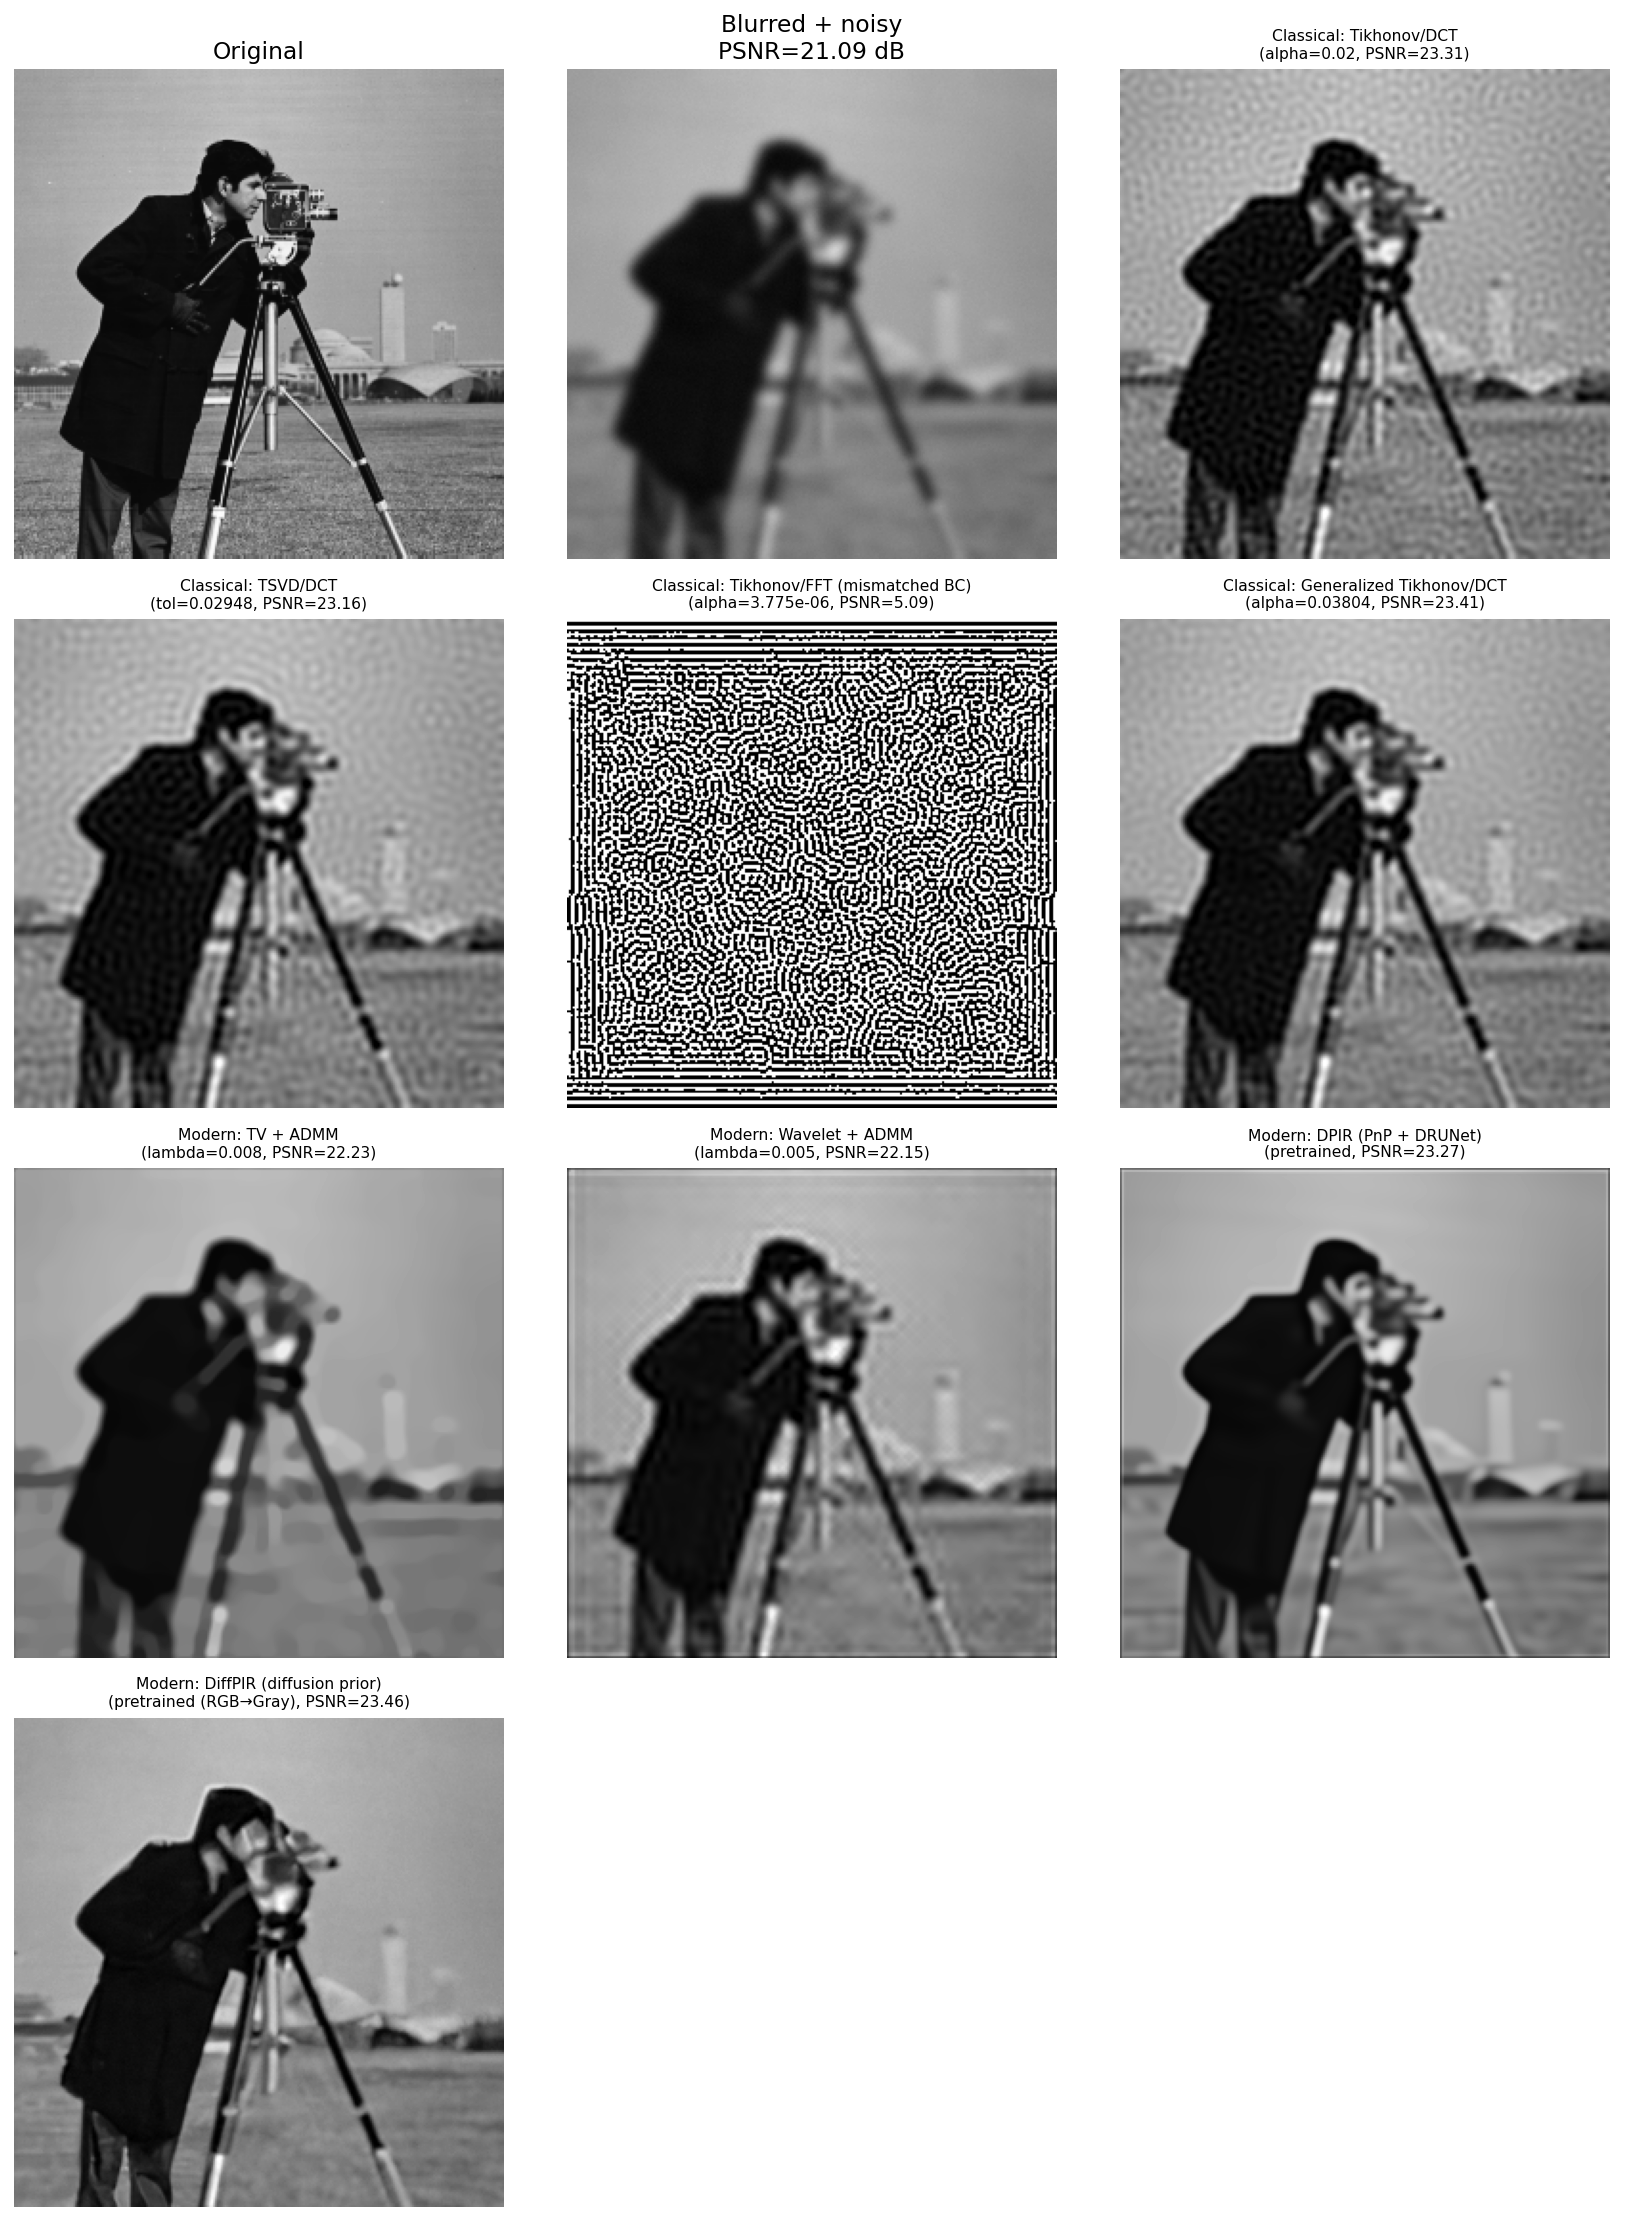
\includegraphics[width=\textwidth]{comparison.png}
% \fbox{\parbox{0.9\textwidth}{\centering\vspace{3cm}
% [Placeholder: Visual comparison of deblurring results for a representative image. \\
% Columns: Ground Truth, Blurred Input, Gen. Tikhonov/DCT, DPIR, DiffPIR]
% \vspace{3cm}}}
\caption{Visual comparison of deblurring results on \textit{a single representative image} from the strong blurring scenario. Classical methods (Generalized Tikhonov) provide the best PSNR but suffer from ringing pattern artifacts, while DiffPIR generates highly realistic textures, achieving the best perceptual quality (LPIPS).}
\label{fig:visual_comparison}
\end{figure}

% ============================================================
\section{Conclusion}
\label{sec:conclusion}

This report has presented an empirical comparison between classical spectral filtering methods and modern learning-based approaches for image deblurring, revealing a landscape in which no single paradigm dominates across all metrics. Among classical methods, generalized Tikhonov regularization with a Laplacian operator consistently emerges as the strongest model-based approach, achieving the best PSNR and relative error at negligible computational cost ($\sim$20--30~ms per image), while the deliberate mismatch experiment with Tikhonov/FFT underscores the critical sensitivity of spectral methods to correctly specified boundary conditions. Modern methods with learned priors clearly excel on perceptual quality: DPIR achieves the best SSIM and strong PSNR by embedding a data-driven denoiser within an optimization loop, and DiffPIR achieves the best LPIPS scores by a wide margin, demonstrating the unique ability of diffusion priors to generate realistic textures even when pixel-wise fidelity is not optimal. A notable finding is that hand-crafted priors (TV, wavelets) solved via ADMM underperform classical spectral methods in our setting, suggesting that in well-posed regimes with known PSF and Gaussian noise, the exact spectral filters with GCV-optimal parameter selection introduce less bias than generic priors constrained by iterative optimization. The divergence among metrics, where Generalized Tikhonov achieves the highest PSNR while degrading SSIM and LPIPS, and DiffPIR sacrifices PSNR for perceptual realism, reinforces the importance of multi-metric evaluation and provides clear practical guidance: classical DCT-based methods remain the default choice for resource-constrained or well-posed settings, DPIR offers the best quality-to-cost tradeoff for general use, and diffusion-based methods are preferred when visual realism is paramount, suggesting a future in which hybrid approaches combining the interpretability of classical optimization with the expressiveness of learned priors will continue to advance the field.

% ── Bibliography ────────────────────────────────────────────
\newpage
\printbibliography[heading=bibintoc]   % includes in TOC

\end{document}